% Introduction

\section{Scope of study}

Firms are obliged to become more innovative to maintain and enhance their competitive advantage in a rapidly evolving and technology\hyp{}driven economy \citep{lubit2001keys,urbancova2013competitive}. Innovation involves inventing, developing, and implementing new ideas that create value for all participants in an innovation ecosystem \citep{garud2013perspectives}. The accelerating pace of technological advances is leading to a proliferation of increasingly complex knowledge and firms can no longer rely solely upon their internal knowledge assets for innovation \citep{chesbrough2009open,enkel2009open}. Consequently, a growing number of firms are embracing \enquote{open innovation} as a competitive strategy \citep{chesbrough2003open,enkel2009open,stanko2017under}. With open innovation, the innovation process relies heavily on accessing, harnessing, and absorbing flows of knowledge across a firm’s boundaries \citep{chesbrough2017future}. \medskip

Tacit knowledge is strongly implicated in innovation as it guides the thought processes that produce novel ideas \citep{leonard1998role,cavusgil2003tacit}. People develop and use tacit knowledge before they are able to formalise or codify it. Thus, the leading edge of the firm’s learning is often to be found in the tacit knowledge of its employees \citep{horvath2000working}. Though tacit knowledge is considered vital for innovation \citep{leonard1998role,von2000enabling,cavusgil2003tacit,amar2008descriptive,seidler2008use}, it has received scant attention in the open innovation literature (see Figure \ref{fig:biblio}). This may be attributed to the fact that tacit knowledge is a mostly hidden resource that is difficult to measure \citep{haldin2000difficulties,jasimuddin2005paradox}. This study addresses this research gap by using mixed\hyp{}method social network analysis to examine the role of tacit knowledge in three open innovation projects. Specific attention is given to the psychosocial factors affecting tacit knowledge exchange, the rationale being that a deeper understanding of such factors should contribute to improved knowledge management practices in open innovation. \medskip

\begin{figure}
    \centering
    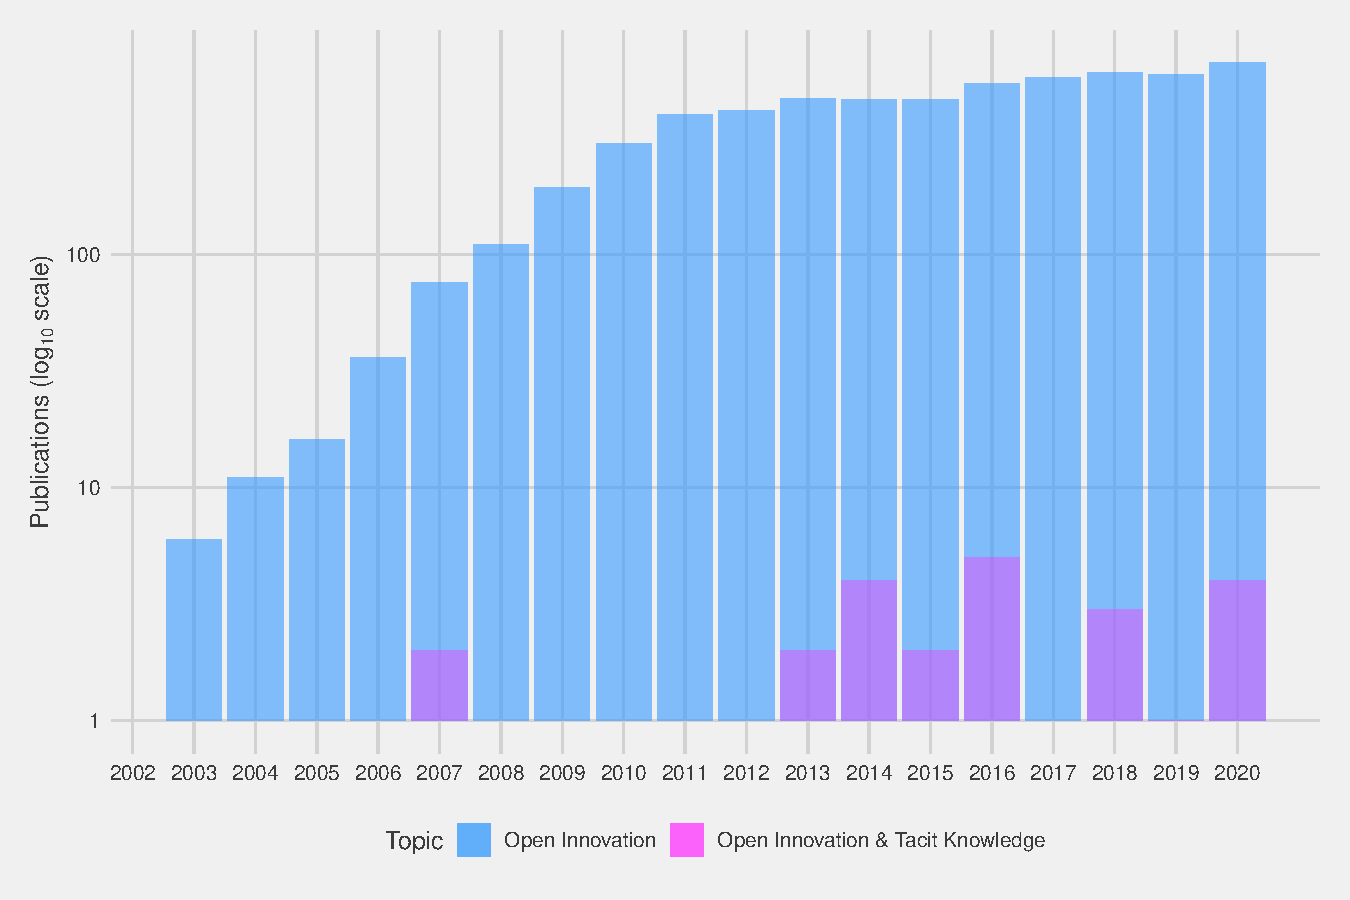
\includegraphics[width=0.7\linewidth]{Images/tk_oi.pdf}
    \caption{Articles published each year on open innovation with the relative proportion of articles referencing tacit knowledge ($log_{10}$ scale). Very few open innovation articles address tacit knowledge directly. Data from Scopus (search query: TITLE-ABS-KEY ("open innovation"), TITLE-ABS-KEY ("tacit knowledge"  AND  "open innovation")).}
    \label{fig:biblio}
\end{figure}

\section{Background}

\subsection{Maintaining competitive advantage}

Proponents of the resource-based view of a firm\footnote{A firm, also referred to as a business, company or enterprise, is an organisation that employs productive resources to obtain products and/or services which are offered in the market with the aim of making a profit.} argue that competitive advantage stems from the application of tangible and intangible resources available to the firm \citep{wernerfelt1984resource,peteraf1993cornerstones}. Moreover, sustained competitive advantage can be achieved if a firm's resources are valuable, rare, inimitable, and non\hyp{}substitutable \citep{barney1991firm}. Because knowledge fuels innovation, it is arguably the most critical resource in today's rapidly evolving and increasingly technology\hyp{}driven economy \citep{grant1996toward,urbancova2013competitive}. Tacit knowledge, in particular, helps a firm resist imitation by competitors because it is embodied in people and embedded in the things they create \citep{horvath2000working}. Moreover, tacit knowledge is quite \enquote{sticky} and thus not easily appropriated \enquote{sticky} \citep{szulanski1996exploring}. While this stickiness does make the mobilisation of tacit knowledge challenging, its appropriation by competitors is much more challenging \citep{horvath2000working}. \medskip

Keeping abreast of rapidly evolving technology demands levels of knowledge beyond what most firms either possess or can develop in a market\hyp{}relevant time frame \citep{enkel2009open}. Open innovation may be defined as a distributed innovation process involving purposely managed knowledge flows across organisational boundaries, using mechanisms in line with the firm's business model \citep{chesbrough2014explicating}. Because open innovation allows firms to access knowledge in a more timely manner, a growing number of firms are embracing open innovation as a competitive strategy \citep{stanko2017under}. The business model helps a firm decide which inflows of knowledge can fuel innovation, and which knowledge should be released to other organisations \citep{chesbrough2017future}. Key benefits of open innovation include timely access to new technology, sharing of risk, reduced costs of development, better customer acceptance of products or services, and enhanced ability to innovate continuously \citep{ye2013exploring}. \medskip
 
 Open innovation can be described in terms of \enquote{inbound}, \enquote{outbound} and \enquote{coupled} innovation processes \citep{gassmann2004towards}. Inbound open innovation enriches a firm’s knowledge base through integrating suppliers, customers and other external actors \citep{xu2013inbound}, whereas outbound open innovation refers to the commercial exploitation of knowledge that has been developed in-house \citep{de2016knowledge}. Coupled open innovation focuses on strategic partnerships that encompass both inbound and outbound innovation processes \citep{spithoven2013open}. Figure \ref{fig:oi_funnel} illustrates how these processes may work in practice. \medskip

\begin{figure}
	\centering
	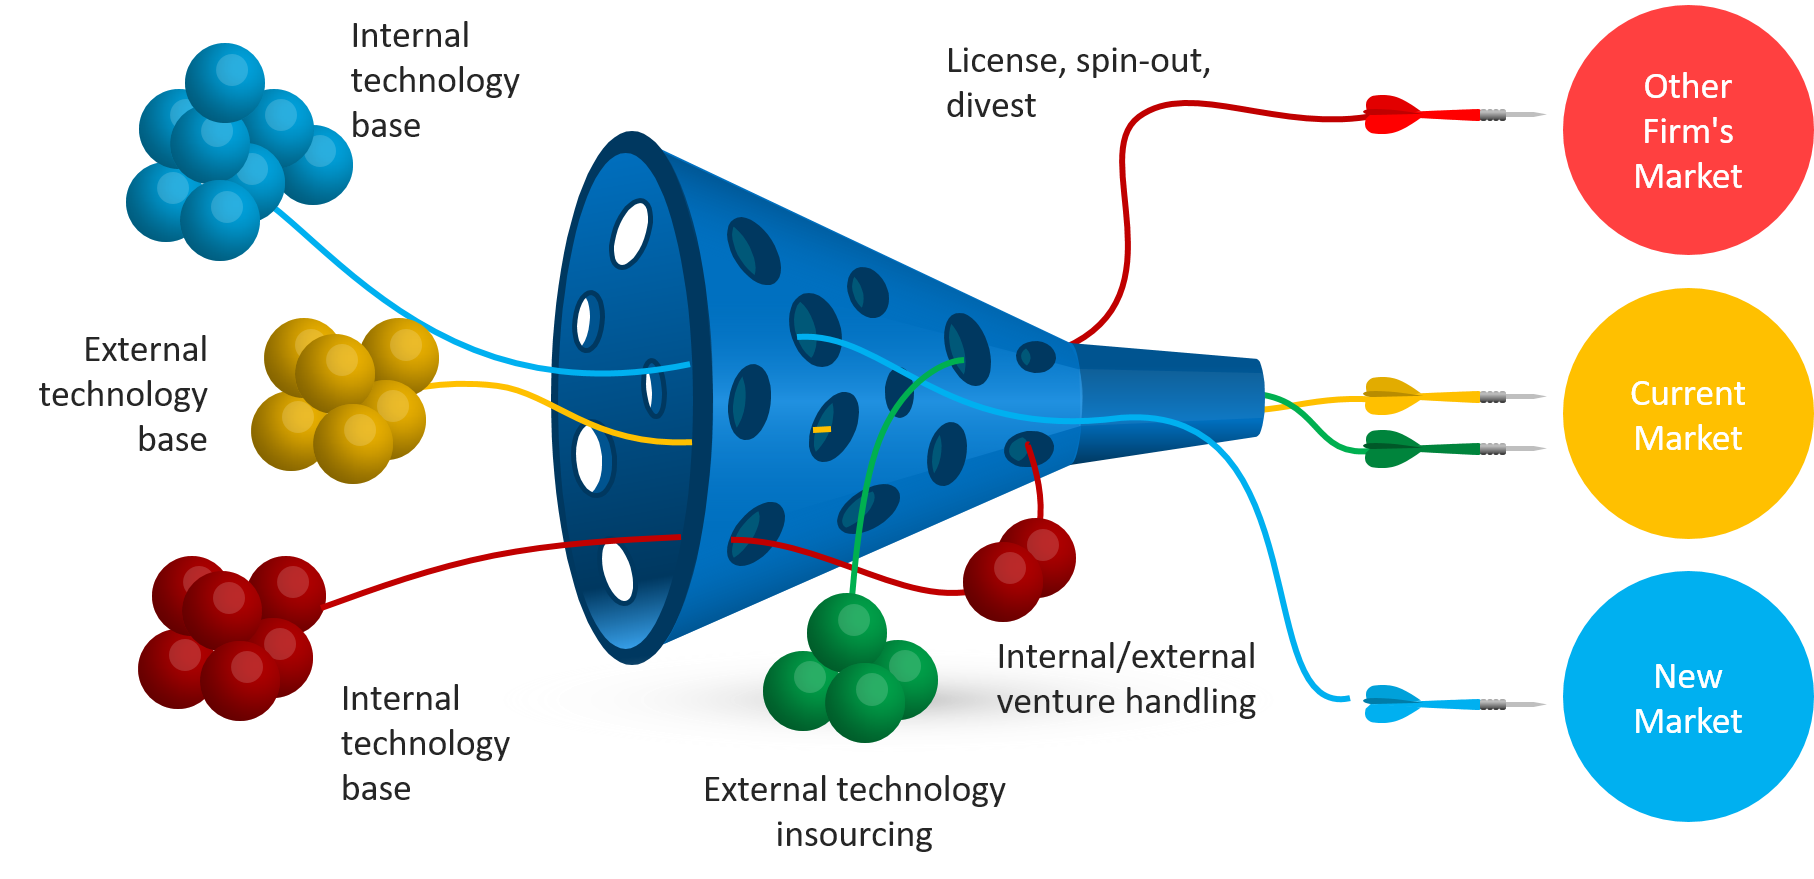
\includegraphics[width=0.9\linewidth]{Images/oi_funnel.png}
	\caption{Open innovation funnel illustrating inbound, outbound, and coupled innovation processes. Open innovation presents multiple pathways for generating value from knowledge. How easily knowledge is able to flow across organisational boundaries depends on the strength of inter-organisational relationships and the absorptive and desorptive capacity of open innovation partner firms \citep{chesbrough2004open,lichtenthaler2010technology}.} 
	\label{fig:oi_funnel}
\end{figure}

 With open innovation, the locus of knowledge creation does not necessarily correspond to the locus of innovation \citep{gassmann2004towards}. For instance, with inbound open innovation, the locus of innovation is inside the firm receiving new external knowledge. This is not the case with outbound open innovation, where the locus of innovation is external to the firm providing knowledge. With coupled open innovation, the locus of innovation straddles firm boundaries, that is, partners share responsibility for achieving a successful innovation outcome. The locus of exploitation (application of knowledge for commercial benefit) can also be different to the locus of innovation. For example, a firm may come up with an innovative solution to a problem through inbound open innovation, but use outbound open innovation for commercial exploitation by a third-party \citep{gassmann2004towards}. All of this has implications for power relations in open innovation partnerships. \medskip

\subsection{Key capabilities for open innovation}

Different capabilities are required for inbound, outbound, and coupled open innovation. Firms pursuing inbound open innovation, for instance, need \enquote{absorptive capacity} to make sense of, and exploit, unfamiliar external knowledge  \citep{vanhaverbeke2007connecting}. Absorptive capacity enhances a firm’s ability to use external knowledge to build other organisational capabilities \citep{zahra2002absorptive,ambrosini2009dynamic,sun2010examination}. In other words, a firm with enhanced absorptive capacity is able to use external knowledge more effectively in response to changes in competitive landscape \citep{chen2009positive,vasylieva2013absorptive,de2016knowledge}. Relative differences in absorptive capacity between open innovation partners can impede knowledge integration, contribute to power imbalances, and undermine alliance performance, all of which can result in sub-optimal open innovation outcomes \citep{lane1998relative,vanhaverbeke2007connecting,zobel2016benefiting,tell2017managing}. Overcoming relative differences in absorptive capacity is crucial for successful open innovation. This requires open innovation partners to have a strong learning orientation to help align thinking and reduce differences in understanding between them  \citep{nooteboom2000learning,sun2010examination,de2016knowledge}. \medskip

Firms wanting to exploit their internally developed knowledge through outbound open innovation require \enquote{desorptive capacity} to identify and act on knowledge transfer opportunities \citep{lichtenthaler2010technology,denford2018absorption}. This includes having appropriate mechanisms for managing and leveraging intellectual property \citep{chesbrough2012open}. Absorptive and desorptive capacity can be seen as \enquote{two sides of the same coin}, i.e. they are pull and push factors governing knowledge transfer processes \citep{dell2015absorptive}. \medskip

Another important capability needed for open innovation is the ability to develop and maintain strong and productive inter\hyp{}organisational networks \citep{chesbrough2012open}. Management efforts to create or widen existing inter\hyp{}organisational networks may be frustrated by people who are either reluctant to form new ties, unwilling to facilitate third\hyp{}party ties, or otherwise change their existing networks \citep{davis2010agency}. For example, negative attitudes such as \enquote{not\hyp{}invented\hyp{}here} and \enquote{not\hyp{}shared\hyp{}here} (also referred to as \enquote{not\hyp{}sold\hyp{}here}) syndromes can undermine efforts to develop and maintain strong and productive knowledge exchange networks in open innovation \citep{lichtenthaler2006attitudes,de2014neither,podmetina2015skills}. Not\hyp{}invented\hyp{}here syndrome refers to resistance within a firm against externally developed knowledge \citep{katz1982investigating,hussinger2011search,antons2015opening}. Not\hyp{}shared\hyp{}here syndrome is a negative attitude towards external exploitation of internally developed knowledge \citep{chesbrough2003open,lichtenthaler2006attitudes,de2014neither}. Not\hyp{}invented\hyp{}here syndrome not only affects the absorptive capacity of the firm receiving external knowledge in inbound open innovation, it also stymies efforts to transfer knowledge to firms in outbound open innovation. In the case of not\hyp{}shared\hyp{}here syndrome, reticence to transfer knowledge out of the firm affects its desorptive capacity \citep{lichtenthaler2006attitudes}. Finding ways to overcome negative attitudes towards knowledge sharing is essential to allow the formation of new and productive relationships that enable knowledge to be recombined in novel ways \citep{nahapiet1998social,obstfeld2005social,davis2010agency,meyer2010rise,hussinger2011search}. \medskip

Developing strong and productive inter\hyp{}organisational networks requires people who can operate effectively across organisational boundaries i.e. people who straddle boundaries, otherwise known as \enquote{boundary spanners}. Effective boundary spanners are not only able to broker new relations that extend or widen existing inter\hyp{}organisational networks, but also play a key role in reducing the cognitive distance between open innovation partners and helping people make sense of complexity \citep{tushman1981boundary,fleming2007brokerage,goffin2010managing}. Moreover, boundary spanners can also help build trust, an important antecedent for knowledge sharing \citep{levin2004strength,renzl2008trust,meyer2010rise,sankowska2013relationships,kucharska2016trust}. \medskip

\subsection{Role of tacit knowledge in open innovation}

Codified or explicit knowledge can be formulated into written sentences, mathematical equations, and other symbols for comprehension. By comparison, tacit knowledge is more complex, ambiguous, and subjective \citep{munoz2015tacit}. Tacit knowledge is accumulated by people through observation, imitation, and repeated interactions i.e. tacit knowledge is deeply rooted in experience \citep{nonaka1995knowledge}. Rather than conceptualising knowledge as either tacit or explicit, it is more appropriate to view knowledge varying along a continuum that ranges from low tacitness (most explicit) to high tacitness (least explicit) \citep{leonard1998role,chuang2016can}. Not only is tacit knowledge embodied in the minds and actions of individuals, it is also inculcated in group practice and culture, usually in the form of unwritten rules and procedures \citep{munoz2015tacit}. Tacit knowledge is arguably a defining feature of the various sub-cultures that exist within a firm. \medskip

Given knowledge lies on a spectrum ranging from low to high tacitness, any knowledge flowing across an organisational boundary will invariably have a tacit component to it. Tacit knowledge often provides important context for making sense of explicit knowledge. This is especially true with respect to specialised or complex knowledge \citep{leonard1998role,argote2000knowledge,szulanski2003sticky,amar2008descriptive}. Such knowledge quickly loses its meaning when considered in the absence of tacit knowledge \citep{amar2008descriptive,seidler2008use}. Neglecting the tacit dimension of inter\hyp{}organisational knowledge exchanges may result in sub-optimal, or even worse, failed open innovation outcomes. \medskip

Mobilising tacit knowledge in open innovation is challenging because individuals or groups are either unaware of the tacit dimension of their knowledge, or are unable to express what they know \citep{polanyi1966tacit,leonard1998role}. An iceberg floating on a sea of consciousness is a useful metaphor for describing a firm's knowledge resource. The exposed tip of the iceberg represents explicit knowledge that is easy to recognise and access. Hidden beneath the surface, is the bulk of the iceberg, representing hard to access tacit knowledge \citep{mcadam1999critical}. Many firms do not appreciate the diversity of their knowledge resource, and consequently lack processes to unlock the potential value of tacit knowledge embodied in the minds and actions of employees \citep{nonaka1994dynamic,horvath2000working}. This seriously limits their ability to innovate. Likewise, the inability to recognise the diversity of knowledge resources in partner firms is also a limiting factor for open innovation. \medskip

\begin{figure}
    \centering
    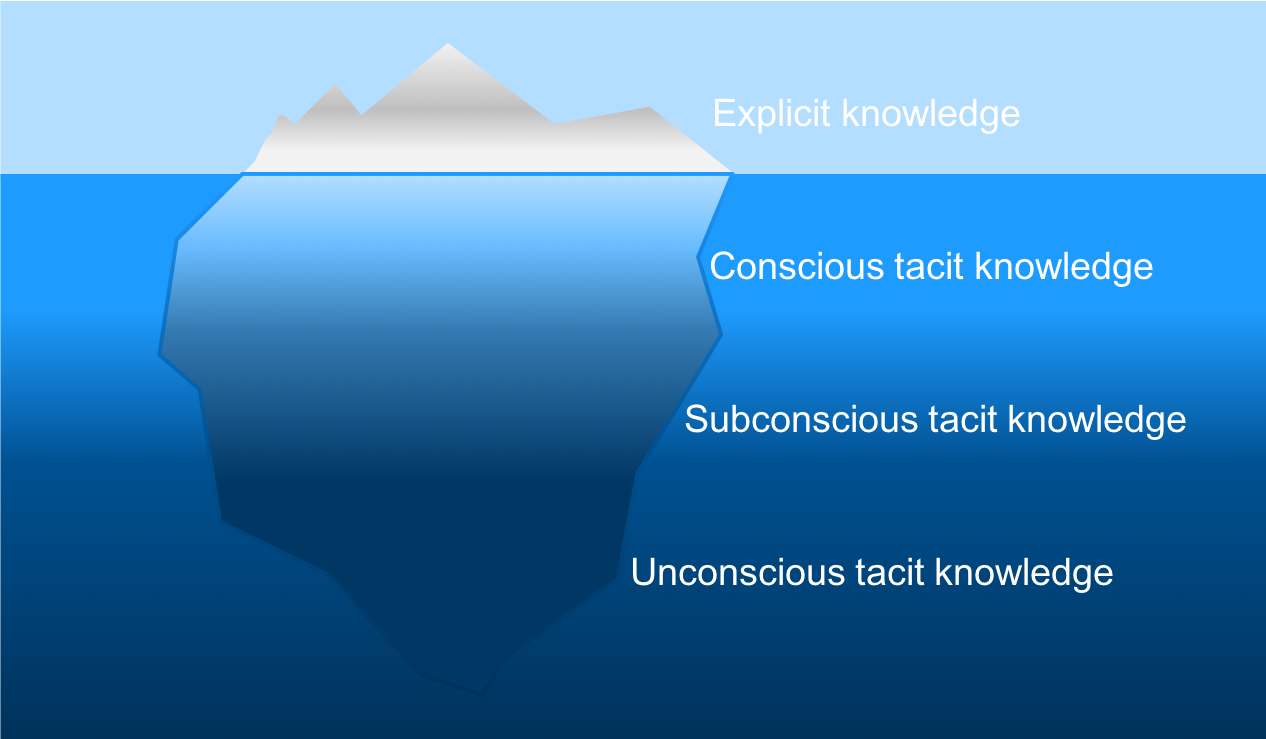
\includegraphics[width=0.7\linewidth]{Images/iceberg.png}
    \caption{An iceberg floating on a sea of consciousness is a useful metaphor for a firm's knowledge resource. Knowledge becomes less visible as one descends deeper into sub-consciousness \citep{haldin2000difficulties}.}
    \label{fig:iceberg}
\end{figure}

Getting people to share their tacit knowledge is not something that can be readily mandated. Sharing happens through volition or free will \citep{polanyi1966tacit}. Individuals or groups are inclined to hoard their knowledge to maintain some form of advantage and are unlikely to disclose their personal or group knowledge if this makes them feel more vulnerable  \citep{levin2004strength,riege2005three,lin2007share,milne2007motivation}. \medskip

Adding to the challenge is the notion that tacit knowledge is not transferred but rather interpreted within a specific context \citep{nonaka1995knowledge,duguid2005art,marabelli2014knowing}. The increasing complexity of knowledge makes interpretation of tacit knowledge that much more difficult \citep{eraut2000non}. Face\hyp{}to\hyp{}face social interaction is key because it allows immediate feedback to confirm understanding and correct any misinterpretations \citep{haldin2000difficulties,gertler2003tacit,koskinen2003tacit}. While advances in information technology (e.g. e\hyp{}mail, instant messaging, video\hyp{}conferencing, and web\hyp{}based collaboration platforms) have made it easier for dispersed team members to communicate with each other, much of this technology is not well-suited for tacit knowledge exchange and immediate feedback. Limited face\hyp{}to\hyp{}face interaction may negatively impact knowledge sharing and idea generation in open innovation \citep{johannessen2001mismanagement}. \medskip

\section{Research opportunity}

\subsection{A network perspective of open innovation}

Knowledge networks represent collections of individuals and teams that come together across organisational, spatial and disciplinary boundaries to create, share or apply a body of knowledge \citep{pugh2013designing}. The business model underpinning open innovation explains how value is generated from inter\hyp{}organisational knowledge networks \citep{chiaroni2010unravelling}. Though tacit knowledge plays a key role in transferring complex knowledge, the extent to which it helps bridge cognitive gaps and stimulate idea generation is poorly understood \citep{seidler2008use}. This may be attributed to invisible nature of tacit knowledge, which makes it especially hard to measure \citep{leonard1998role,haldin2000difficulties}. Because specialised or complex knowledge is likely to have a sizeable tacit component, it has a significant influence on a firm's absorptive and innovative capacity. For this reason tacit knowledge warrants much more attention than it has received in the open innovation literature so far. \medskip

Since tacit knowledge exchange is a socially intensive process, there is merit in using mixed\hyp{}method social network analysis to assess tacit knowledge flows in open innovation \citep{leonard1998role,busch2000graphically,zhu2007social}. Mixed\hyp{}method social network analysis enables the exploration of network structure while not forsaking the qualitative observations about what is going on within a network e.g. influence of organisation culture or sub-cultures and power relations \citep{crossley2010social}. Such analysis can provide useful insights into both endogenous (inherent) and exogenous (environmental) factors influencing tacit knowledge transfer processes \citep{kolleck2013social,tortoriello2015social}. \medskip

\subsection{Exploring motivational factors}

Tacit knowledge requires significantly more effort to communicate than explicit knowledge. People must be sufficiently motivated to seek out and share tacit knowledge \citep{leonard1998role}. Past studies show a significant and positive relation between an individual's level of intrinsic motivation and the amount of tacit knowledge they share \citep[e.g.][]{osterloh2000motivation,kaser2001knowledge,smith2001role}. Intrinsic motivation is about engaging in activities because these are enjoyable or personally meaningful \citep{ryan2000intrinsic}. Although these studies highlight the importance of personal motivation, the psychosocial processes underpinning tacit knowledge exchange and how this impacts open innovation are not well understood. This indicates a need to investigate how personal motivation shapes the development of knowledge sharing relations. \medskip

\subsection{Unpacking power-relations} 

The current literature on power is dominated by two contrasting views of power, namely \enquote{power as domination}, also referred to as \enquote{power\hyp{}over}, and \enquote{power as empowerment}, often characterised as \enquote{power\hyp{}to} \citep{haugaard2012rethinking}. Though it is often stated that \enquote{knowledge is power}, not much is written about power and power\hyp{}relations in the knowledge management literature \citep{haugaard2012rethinking}. People accumulate tacit knowledge to empower themselves in their quest for competence or personal mastery \citep{endres2007tacit}. By sharing their tacit knowledge, individuals are essentially empowering others so that they can perform work more independently and confidently \citep{bordum2002tacit,lin2007share}. Some people may be reluctant to share their hard-earned tacit knowledge if they believe this will compromise or disempower them. \medskip

The network perspective treats power as inherently relational \citep{ibarra1993power}. Actors that bridge otherwise disconnected parts on an inter\hyp{}organisational network are said to occupy \enquote{structural holes} \citep{burt1992structural}. Such actors, also referred to as \enquote{boundary spanners} or \enquote{network brokers}, play a key role in open innovation as they broker new relations, coordinate interactions between partners, and help people make sense of complex or specialised knowledge. They are able to exert considerable influence over information exchange or resource flows. Brokerage may be defined as the \enquote{behaviour by which an actor influences,
manages, or facilitates interactions between other actors} \citep{obstfeld2014brokerage}. One can assess how open innovation partners exercise power by examining patterns of brokerage in knowledge networks. The patterns should reveal who is being empowered through knowledge exchanges and highlight which brokerage mechanisms are the most significant in an open innovation partnership. \medskip

\section{Study objectives}

This study explores tacit knowledge sharing in three open innovation partnerships. Attention is focused on how people are motivated to share tacit knowledge and what patterns of social interaction tell us about tacit knowledge sharing processes in open innovation. The study also examines the organisational context in which tacit knowledge sharing takes place. Four research questions are addressed in this study: \medskip

% \begin{description}
    \begin{enumerate}
        \item To what extent does personal motivation drive tacit knowledge sharing in open innovation?
	    \item What does the structure of tacit knowledge networks reveal about trust and power relations in open innovation partnerships?
	    \item What is the relationship between tacit knowledge sharing and idea generation in open innovation partnerships?
	    \item To what extent do governance structures influence tacit knowledge sharing in open innovation partnerships?
    \end{enumerate}
% \end{description}

The study employs sociocentric network analysis\footnote{Sociocentric network analysis examines an entire network, whereas egocentric network analysis examines an individual's personal network.}, namely exponential random graph modelling, to (a) assess how individual attributes, such as the level and type of personal motivation, educational background, and work experience drive the emergence of tacit knowledge sharing relations, (b) determine whether tacit knowledge sharing is more likely or less likely to happen in the presence of other ties, and (c) examine what patterns of brokerage reveal about power-relations in tacit knowledge networks. This analysis is complemented by semi\hyp{}structured interviews that capture the industrial, organisational, and cultural contexts governing the emergence of collaborative social structures that support tacit knowledge sharing. \medskip  

\section{Research contribution}

This study advances knowledge in two ways. Firstly, the study provides fresh insight into how tacit knowledge sharing facilitates learning and idea generation in open innovation partnerships. Secondly, it breaks new ground by examining how brokerage roles vary according to the amount of tacit knowledge being exchanged and what this means in terms of power relations. By embracing a social network perspective, this study draws attention to key social processes affecting tacit knowledge flows in open innovation. This should help managers devise more effective strategies for transferring complex or specialised (sticky) knowledge across organisational boundaries. Thanks to a lack of clear methodological guidelines, approaches to mixed\hyp{}method social network analysis vary considerably. Another contribution of this study will be the development and testing of a more robust framework for mixed\hyp{}method social network analysis that others can use.    \medskip

\section{Document structure}

The remainder of this document is organised as follows:

\begin{itemize}[leftmargin=0pt]
    \item[] \textbf{Chapter Two} provides a brief overview of social networks and social network analysis and explores key features of knowledge exchange networks.
    \item[] \textbf{Chapter Three} reviews key literature on motivation, trust, and power relevant to tacit knowledge sharing and presents a number of propositions that inform the subsequent analysis.
    \item[] \textbf{Chapter Four} describes the research methodology underpinning this study. This includes an explanation of the rationale for the hybrid mixed\hyp{}method research design used in this study and details of the quantitative and qualitative procedures used to collect and analyse data.
    \item[] \textbf{Chapter Five} presents the results from each case study. For each case, there is a brief description of the open innovation challenge (case overview), followed by network visualisations, exponential random graph modelling results, and results of the analysis of the semi-structured interviews.
    \item[] \textbf{Chapter Six} compares and contrasts the results of each case study and discusses the implications for managing tacit knowledge flows in open innovation partnerships. 
    \item[] \textbf{Chapter Seven} summarises the main findings of this study and reflects on some key lessons learned as this study unfolded. This includes descriptions of the study's limitations and possible avenues for future research. 
\end{itemize}

% affects knowledge sharing behaviour differs according to the level of tacit knowledge being exchanged.

% Actors in knowledge networks are both keepers of knowledge and agents that seek out, communicate, and create knowledge \citep{phelps2012knowledge}. 


% Examining the configuration of social ties in knowledge networks can shed light on the social processes that transform new knowledge into innovations. \medskip

% Actors that know each other well are said to have strong ties with one another. Such actors tend to have similar interests and are privy to the same knowledge. Strong ties tend to make people look inward and not be very receptive to external knowledge. Casual acquaintances, on the other hand, can be regarded as weak ties. Because acquaintances usually mix in different social circles, weak ties are more likely to provide actors access to new knowledge and opportunities \citep{granovetter1973strength}. Actors who bridge otherwise disconnected parts of the knowledge network are termed knowledge brokers. Brokerage may be defined as the \enquote{behaviour by which an actor influences, manages, or facilitates interactions between other actors} \citep{obstfeld2014brokerage}. Knowledge brokers make connections between those who need knowledge and those who have it \citep{davenport1998successful}. They are able to identify and establish strategic relationships with keepers of knowledge. Some knowledge brokers exploit this to their own advantage while others try establish new relations between otherwise disconnected people \citep{gould1989structures,burt1992structural,obstfeld2014brokerage}. \medskip

%  \medskip



% Open Innovation implies an extensive use of inter-organisational relationships to gain access to new external knowledge and to exploit novel ideas \citep{chiaroni2010unravelling}. 


% \subsection{Knowledge networks}

% Knowledge networks represent collections of individuals and teams who come together across organisational, spatial and disciplinary boundaries to create, share or apply a body of knowledge \citep{pugh2013designing}.  Open innovation partnerships may thus be characterised as knowledge networks with an abundance of weak ties. 


